% !Mode:: "TeX:UTF-8"
% \textbf{计算专题------取值说理,与不等式结合}

\begin{defproblem}{T16-A01-01}%
\begin{onlyproblem}%
先化简$\left(1-\dfrac{3}{x+2}\right)\div \dfrac{x^2-2x+1}{x^2-4}$,然后从不等式$2x-6<0$的非负整数解中,选取一个合适的解代入求值.
\end{onlyproblem}%
\begin{onlysolution}%
% \begin{center}
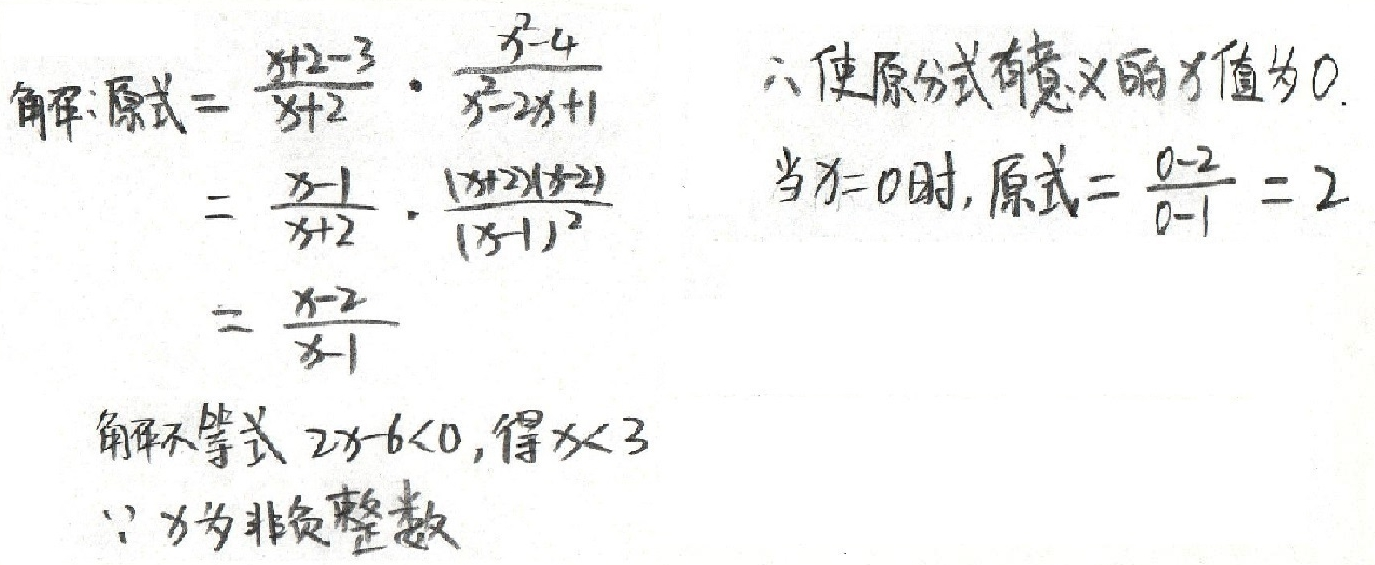
\includegraphics[width=8cm]{T16-A01-01.jpg}
% \end{center}
\end{onlysolution}%
\end{defproblem}


\begin{defproblem}{T16-A01-02}%
\begin{onlyproblem}%
先化简:$\left(\dfrac{1}{x-1}-1\right)\div \dfrac{x^2-2x}{x^2-1}$,然后从不等式组$\left\{\begin{array}{@{}l}
-x+1\le 3\\
2x<4\\
\end{array}\right.$的解集中,选取一个你认为符合题意的$x$的值代入求值.
\end{onlyproblem}%
\begin{onlysolution}%
\begin{center}
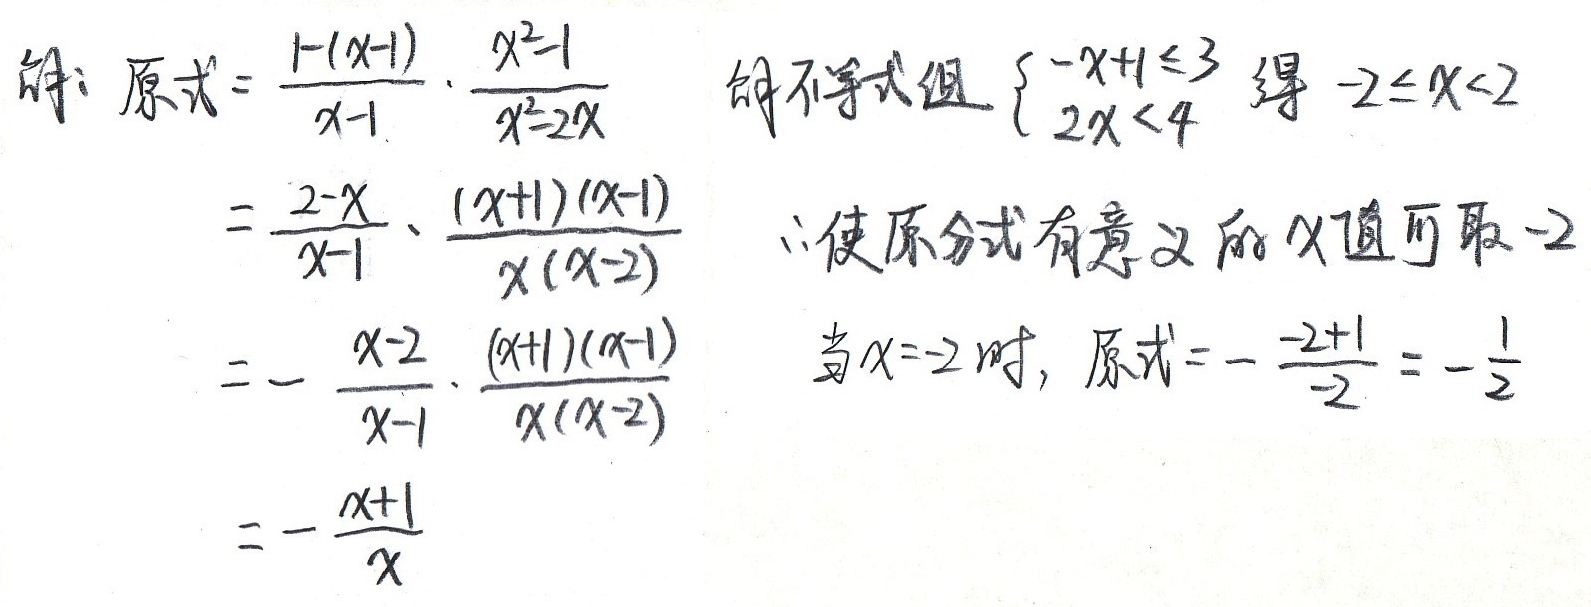
\includegraphics[width=.69\columnwidth]{T16-A01-02.jpg}
\end{center}
\end{onlysolution}%
\end{defproblem}


\begin{defproblem}{T16-A01-03}%
\begin{onlyproblem}%
先化简:$\dfrac{x^2-4x+4}{x^2-2x}\div\left(x-\dfrac{4}{x}\right)$,然后从$-\sqrt 5 <x<\sqrt 5 $的范围内选取一个合适的整数作为$x$的值代入求值.
\end{onlyproblem}%
\begin{onlysolution}%
\begin{center}
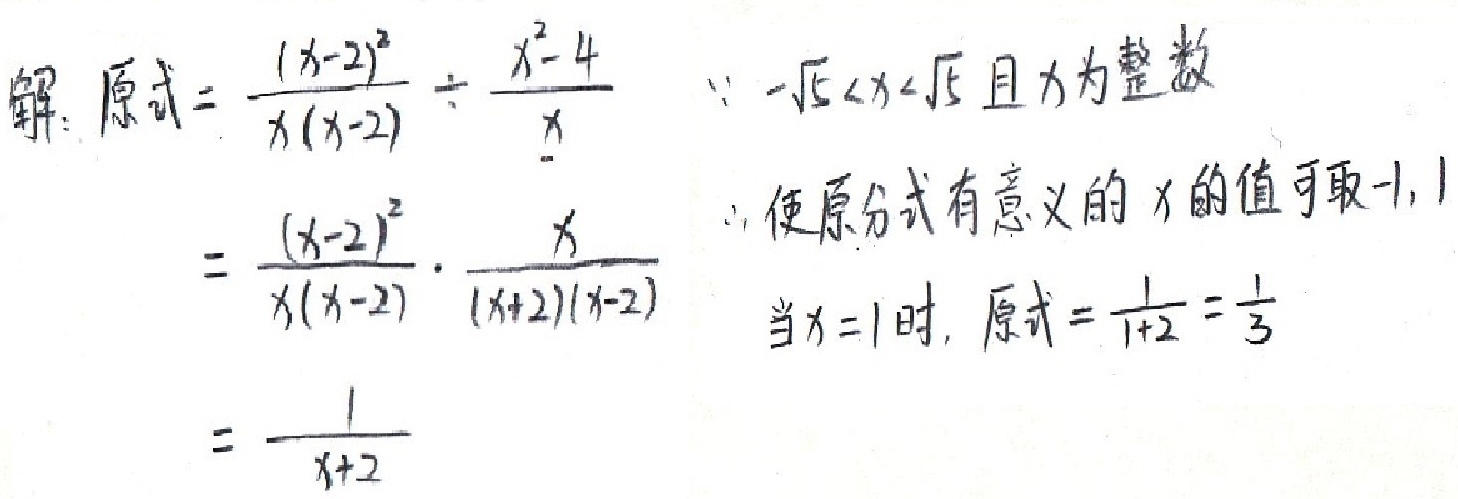
\includegraphics[width=.69\columnwidth]{T16-A01-03.jpg}
\end{center}
\end{onlysolution}%
\end{defproblem}


\begin{defproblem}{T16-A01-04}%
\begin{onlyproblem}%
先化简:$\dfrac{x+3}{x^2-2x+1}\cdot\left(\dfrac{x}{x+3}-\dfrac{x-3}{x^2-9}\right)$,再从不等式组$\left\{\begin{array}{@{}l}
3x-6\le x\\
\dfrac{4x+5}{10}<\dfrac{x+1}{2}\\
\end{array}\right.$的整数解中选择一个合适的数,求出此代数式的值.
\end{onlyproblem}%
\begin{onlysolution}%
\begin{center}
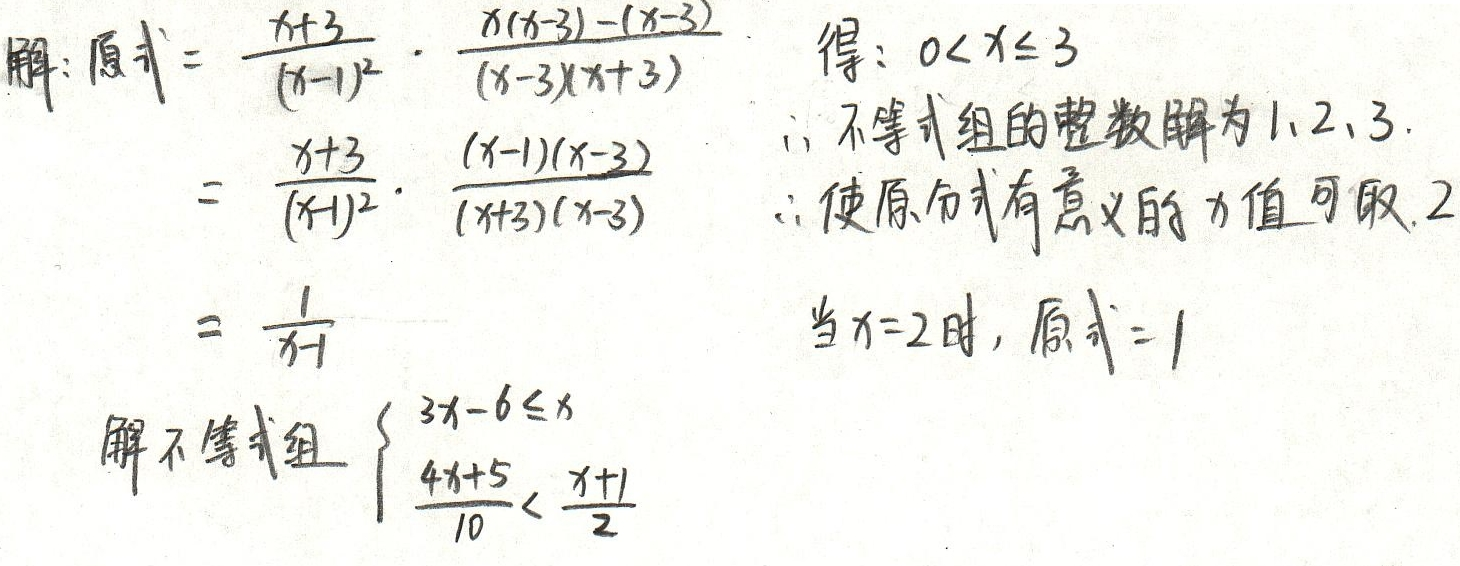
\includegraphics[width=.69\columnwidth]{T16-A01-04.jpg}
\end{center}
\end{onlysolution}%
\end{defproblem}


\begin{defproblem}{T16-A01-05}%
\begin{onlyproblem}%
已知$A=(x-3)\div \dfrac{(x+2)(x^2-6x+9)}{x^2-4}-1$.

(1)化简$A$;

(2)若$x$满足不等式组$\left\{\begin{array}{@{}l}
 2x-1<x\\
 1-\dfrac{x}{3}<\dfrac{4}{3}\\
 \end{array}\right.$且$x$为整数时,求$A$的值.
\end{onlyproblem}%
\begin{onlysolution}%
\begin{center}
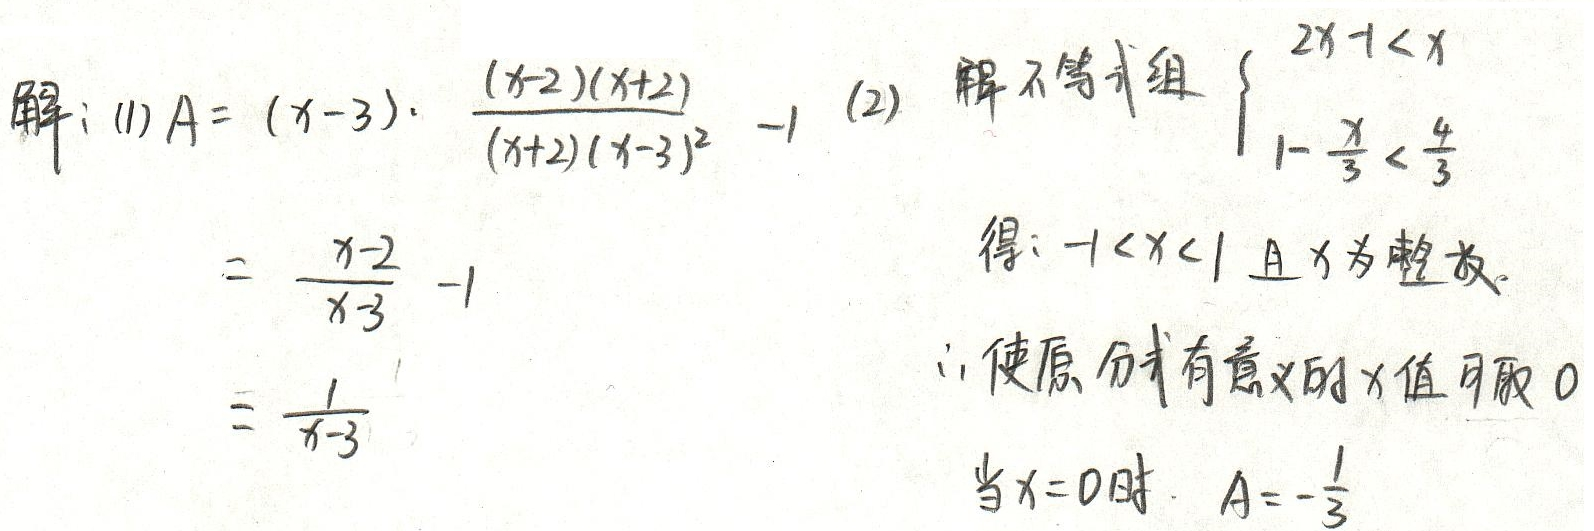
\includegraphics[width=.69\columnwidth]{T16-A01-05.jpg}
\end{center}
\end{onlysolution}%
\end{defproblem}


\begin{defproblem}{T16-A01-06}%
\begin{onlyproblem}%
有三个代数式:①$a^{2}-2ab+b^{2}$,②$2a-2b$,③$a^{2}-b^{2}$,其中$a\neq b$.


(1)请你从①②③三个代数式中任意选取两个代数式,分别作为分子和分母构造成一个分式;

(2)请把你所构造的分式进行化简;

(3)若$a$,$b$为满足不等式$0<x<3$的整数解,且$a>b$,请求出化简后的分式的值.

\end{onlyproblem}%
\begin{onlysolution}%
\begin{center}
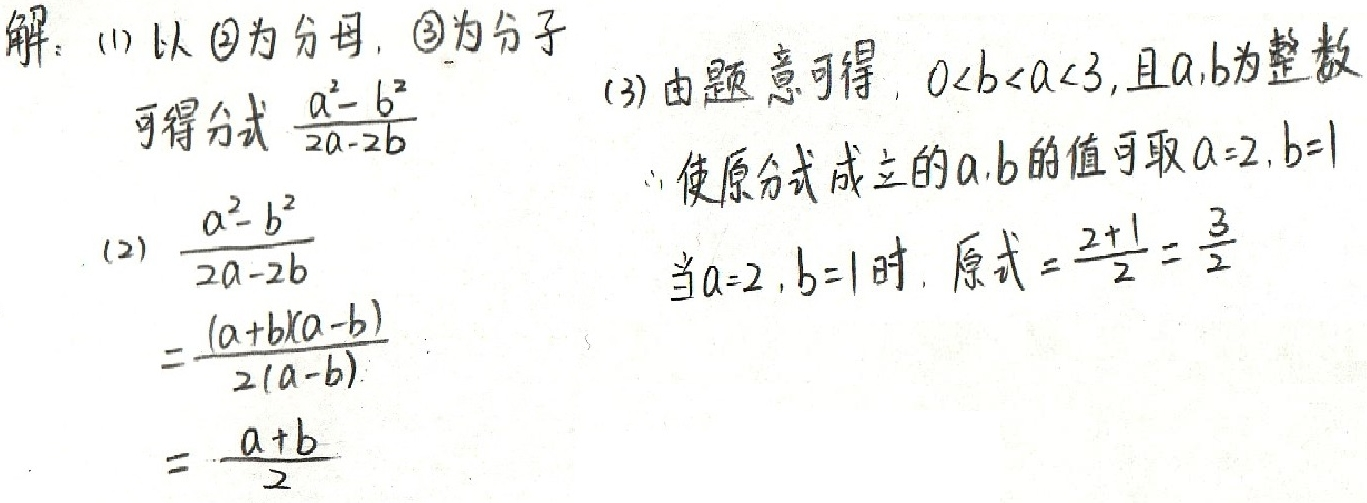
\includegraphics[width=.69\columnwidth]{T16-A01-06.jpg}
\end{center}
\end{onlysolution}%
\end{defproblem}



\begin{defproblem}{T16-A01-07}%
\begin{onlyproblem}%
已知关于$x$的方程$x^2-2ax+a=0$有两个相等的实数根,请先化简代数式$\left(\dfrac{1}{a-1}-\dfrac{1}{a+1}\right)\div \dfrac{2}{a+1}$,并求出该代数式的值.

\end{onlyproblem}%
\begin{onlysolution}%
% \begin{center}
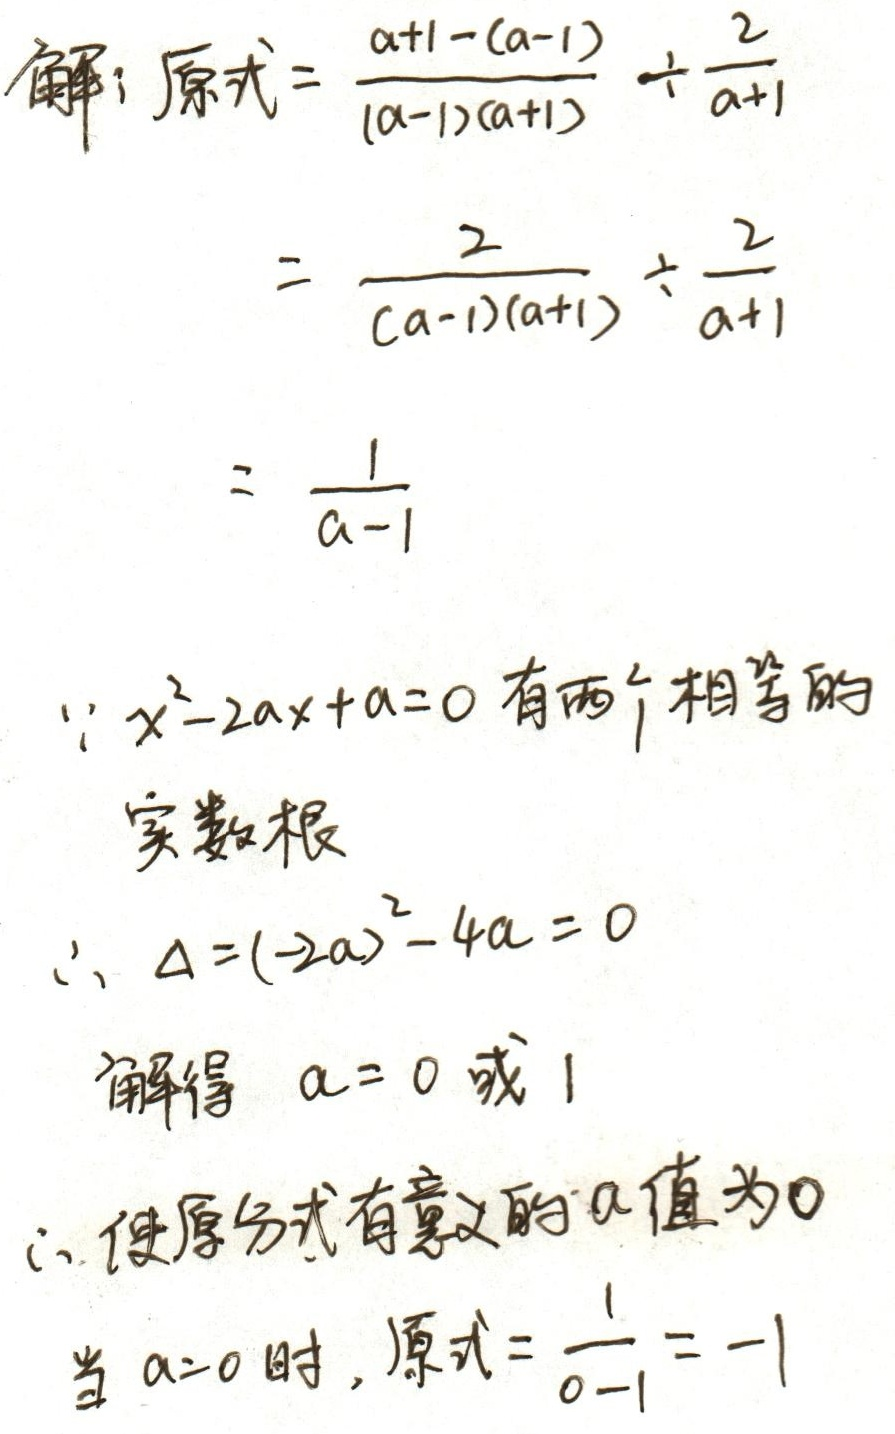
\includegraphics[width=5cm]{T16-A01-07.jpg}
% \end{center}
\end{onlysolution}%
\end{defproblem}


\begin{defproblem}{T16-A01-08}%
\begin{onlyproblem}%
先化简,再求代数式$\dfrac{a^2+a}{a^2+2a+1}\div \left(1+\dfrac{1}{a-1}\right)$的值,其中$a=2\tan60^{\circ}-1$.

\end{onlyproblem}%
\begin{onlysolution}%

\end{onlysolution}%
\end{defproblem}

